\hypertarget{a00834}{}\section{Digi\+Trace Guide}
\label{a00834}\index{DigiTrace Guide@{DigiTrace Guide}}
How to add tracing to your plug-\/ins and view logging from the plug-\/in host. 

\hypertarget{a00834_digitrace__contents}{}\subsection{On this page}\label{a00834_digitrace__contents}
\begin{DoxyItemize}
\item \mbox{\hyperlink{a00834_digitrace__intro}{What is Digi\+Trace?}} \item \mbox{\hyperlink{a00834_digitrace__quickstart}{Digi\+Trace quick start guide}} \item \mbox{\hyperlink{a00834_digitrace__logfiles}{Digi\+Trace log files}} \item \mbox{\hyperlink{a00834_digitrace__configuring}{Configuring Digi\+Trace}} \item \mbox{\hyperlink{a00834_digitrace__bonus_features}{Bonus features}} \item \mbox{\hyperlink{a00834_digitrace__tracingfromplugins}{Adding traces to an A\+AX plug-\/in}} \item \mbox{\hyperlink{a00834_digitrace__advancedconfiguration}{Advanced Digi\+Trace configuration}} \item \mbox{\hyperlink{a00834_digitrace__compatibility}{Compatibility}} \item \mbox{\hyperlink{a00834_digitrace__additionalinformation}{Additional Information}}\end{DoxyItemize}
 \hypertarget{a00834_digitrace__intro}{}\subsection{What is Digi\+Trace?}\label{a00834_digitrace__intro}
 Digi\+Trace is a logging tool used by many Avid audio applications. Digi\+Trace provides high-\/performance, real-\/time tracing capabilities and can help you debug hard-\/to-\/isolate problems in real-\/time code. Pro Tools and other Avid audio products are instrumented with Digi\+Trace, and it is easy to add Digi\+Trace logging to your A\+AX plug-\/ins.

 This document outlines how to use Digi\+Trace, both as a developer to add trace instrumentation to your code and as an end user to view or record trace instrumentation for an instrumented application.

\hypertarget{a00834_digitrace__intro__whatdoesitdo}{}\subsubsection{What does Digi\+Trace do?}\label{a00834_digitrace__intro__whatdoesitdo}
 Digi\+Trace generates encrypted logs on users\textquotesingle{} systems. These log files can be decrypted via the Digi\+Trace\+Decryptor application that is included in the Digi\+Trace Tools package.

 By default, Digi\+Trace logs basic information including details about the system, software, component versions, and any errors that are encountered. By using a simple configuration text file, Digi\+Trace can be easily configured to provide additional logging information such as plug-\/in loading details. Here are some examples of how you can use Digi\+Trace\+:

 
\begin{DoxyItemize}
\item You can use Digi\+Trace in your plug-\/ins when you need a convenient, high-\/performance logging solution.  
\item You can use the default Digi\+Trace logs that Pro Tools generates to help you understand problems that your plug-\/ins encounter when running on Pro Tools.  
\item You can add Digi\+Trace statements and stack traces to your released plug-\/ins in order to help you troubleshoot end-\/user issues more quickly.  
\item You can (and should!) submit Digi\+Trace logs when reporting bugs and other Pro Tools issues to Avid.  
\end{DoxyItemize}



 \hypertarget{a00834_digitrace__quickstart}{}\subsection{Digi\+Trace quick start guide}\label{a00834_digitrace__quickstart}
 This section provides quick steps for the following common tasks\+: \begin{DoxyItemize}
\item \mbox{\hyperlink{a00834_digitrace__gettingstarted__logfiles}{Find and decrypt Digi\+Trace log files}} \item \mbox{\hyperlink{a00834_digitrace__gettingstarted__config}{Configure Digi\+Trace for A\+AX plug-\/in logging}} \item \mbox{\hyperlink{a00834_digitrace__gettingstarted__configurefordevelopment}{Configure Digi\+Trace for plain-\/text output}} \item \mbox{\hyperlink{a00834_digitrace__gettingstarted__addingtracing}{Add tracing to a plug-\/in}}\end{DoxyItemize}
\hypertarget{a00834_digitrace__gettingstarted__logfiles}{}\subsubsection{Find and decrypt Digi\+Trace log files}\label{a00834_digitrace__gettingstarted__logfiles}
 Digi\+Trace log files are placed into a common logs directory. The specific directory that is used depends on the version of Digi\+Trace -\/ see \mbox{\hyperlink{a00834_digitrace__logfiles__wherearethelogs}{Where are Digi\+Trace log files stored?}}

 By default, the version of Digi\+Trace that is installed with Avid audio products generates logs in an encrypted format with the extension \char`\"{}.\+dlog\char`\"{}. Developer builds of Pro Tools and other applications are configured to generate plain-\/text logs.

 You can convert .dlog files to plain-\/text using the Digi\+Trace\+Decryptor tool that is included in the Digi\+Trace Tools package available for download from the Avid developer portal. To decrypt a log using this tool, simply drag-\/and-\/drop the .dlog file onto the tool. You can also set this tool as the default application for opening .dlog files in your OS, which will allow you to decrypt and open .dlog files directly.

\hypertarget{a00834_digitrace__gettingstarted__config}{}\subsubsection{Configure Digi\+Trace for A\+A\+X plug-\/in logging}\label{a00834_digitrace__gettingstarted__config}
 You must customize the Digi\+Trace configuration to enable extra logging, such as debug logging for \mbox{\hyperlink{a00852}{A\+AX}} plug-\/ins.

 Digi\+Trace uses a plain-\/text configuration file to enable custom logging. This file uses the suffix \char`\"{}.\+digitrace\char`\"{} and is located within or beside the application. For example, the configuration files for Pro Tools are located at\+:
\begin{DoxyItemize}
\item OS X\+: Pro Tools.\+app/\+Contents/\+Resources/config.digitrace
\item Windows\+: C\+:\textbackslash{}Program Files\textbackslash{}Avid\textbackslash{}Pro Tools\textbackslash{}Pro\+Tools.\+digitrace
\end{DoxyItemize}

 To configure Digi\+Trace to print logs from \mbox{\hyperlink{a00395_ab53f1d6a94f8b6ebb3a101f71bfe4e82}{A\+A\+X\+\_\+\+T\+R\+A\+CE}} or \mbox{\hyperlink{a00395_ac2aa820ece56bb59140ad561218db4b3}{A\+A\+X\+\_\+\+T\+R\+A\+C\+E\+\_\+\+R\+E\+L\+E\+A\+SE}} macros in \mbox{\hyperlink{a00852}{A\+AX}} plug-\/ins, add the following line to the .digitrace configuration file for the application\+:

 D\+T\+F\+\_\+\+A\+A\+X\+P\+L\+U\+G\+I\+NS=file@D\+T\+P\+\_\+\+L\+O\+W\+E\+ST 

 If a config.\+digitrace file does not already exist for a Digi\+Trace-\/enabled application then you can create it to enable Digi\+Trace. For more information about customizing the Digi\+Trace configuration and enabling different levels of debug logging, see \mbox{\hyperlink{a00834_digitrace__configuring}{Configuring Digi\+Trace}} .

\hypertarget{a00834_digitrace__gettingstarted__configurefordevelopment}{}\subsubsection{Configure Digi\+Trace for plain-\/text output}\label{a00834_digitrace__gettingstarted__configurefordevelopment}
 In order to be able to view streaming log output in real time, Digi\+Trace must be configured for plain-\/text output. This is the default configuration for developer builds of Pro Tools and other Avid audio applications.

 To configure shipping applications for plain-\/text log output, you must replace the application\textquotesingle{}s installed Digi\+Trace library with a development version of the Digi\+Trace library. Development builds of Digi\+Trace are included in the Digi\+Trace Tools package. Search for \char`\"{}\+Digitrace.\+framework\char`\"{} on OS X or \char`\"{}\+Digi\+Trace.\+dll\char`\"{} on Windows and replace the installed shipping version of the library with the developer version from the Digi\+Trace Tools package to configure the application for plain-\/text output.

 Note that the developer version of Digi\+Trace may output logs to a different directory than the shipping version. In general, developer builds of Digi\+Trace will place log files in a directory next to the instrumented application. For example, developer builds of Pro Tools will output logs to a logs directory placed adjacent to the Pro Tools application bundle rather than in the user\textquotesingle{}s Library/\+Logs/\+Avid folder.

\hypertarget{a00834_digitrace__gettingstarted__addingtracing}{}\subsubsection{Add tracing to a plug-\/in}\label{a00834_digitrace__gettingstarted__addingtracing}
 To easily add tracing to an \mbox{\hyperlink{a00852}{A\+AX}} plug-\/in, use the \mbox{\hyperlink{a00395_ab53f1d6a94f8b6ebb3a101f71bfe4e82}{A\+A\+X\+\_\+\+T\+R\+A\+CE}} or \mbox{\hyperlink{a00395_ac2aa820ece56bb59140ad561218db4b3}{A\+A\+X\+\_\+\+T\+R\+A\+C\+E\+\_\+\+R\+E\+L\+E\+A\+SE}} macros. Logging from the \char`\"{}release\char`\"{} macro will be enabled for all builds of the plug-\/in, whereas logging from the \char`\"{}standard\char`\"{} macro will only be enabled in Debug builds of the plug-\/in.



 \hypertarget{a00834_digitrace__logfiles}{}\subsection{Digi\+Trace log files}\label{a00834_digitrace__logfiles}
 The default logging in Avid audio applications includes data that can be useful in many different troubleshooting situations. For example\+:


\begin{DoxyItemize}
\item Information about the user\textquotesingle{}s system configuration
\item A complete list of loaded components and libraries. (If the user has an old or incompatible version of your plug-\/ins installed on his system, you will know about it!)
\item Crash logs in the event of a system failure
\end{DoxyItemize}

 In addition, you can add Digi\+Trace logging code to your plug-\/ins, helping you examine potential issues in the way your plug-\/in is running on a user\textquotesingle{}s computer even when you cannot reproduce the issue locally.

\hypertarget{a00834_digitrace__logfiles__wherearethelogs}{}\subsubsection{Where are Digi\+Trace log files stored?}\label{a00834_digitrace__logfiles__wherearethelogs}
 \hypertarget{a00834_digitrace__logfiles__wherearethelogs__directory}{}\paragraph{Log directory}\label{a00834_digitrace__logfiles__wherearethelogs__directory}
 Digi\+Trace logs are stored in a log files directory on the user\textquotesingle{}s system. The default location of this directory depends on the operating system and on which version of Digi\+Trace is being used\+:

 
\begin{DoxyItemize}
\item Pro Tools / Digi\+Trace 11.\+0 and later\+: $\sim$/\+Library/\+Logs/\+Avid/ (OS X)  C\+:\textbackslash{}Program Files\textbackslash{}Avid\textbackslash{}Pro Tools\textbackslash{}Logs (Windows)   
\item Pro Tools / Digi\+Trace 9.\+0 -\/ 10.\+3\+: $\sim$/\+Library/\+Logs/\+Avid\+Log\+Files/ (OS X)  C\+:\textbackslash{}Users\textbackslash{}\mbox{[}username\mbox{]}\textbackslash{}Avid\+Log\+Files\textbackslash{} (Windows 7 or Windows 8)  C\+:\textbackslash{}Documents and Settings\textbackslash{}\mbox{[}username\mbox{]}\textbackslash{}Avid\+Log\+Files\textbackslash{} (Windows XP)   
\item Pro Tools / Digi\+Trace 8.\+0.\+3 -\/ 8.\+5\+: \mbox{[}Pro Tools application directory\mbox{]}/\+Log\+Files/ (All configurations)   
\end{DoxyItemize}

 This default log directory can be overridden in the Digi\+Trace config file. See \mbox{\hyperlink{a00834_digitrace__advancedconfiguration}{Advanced Digi\+Trace configuration}} for more information.

\hypertarget{a00834_digitrace__logfiles__wherearethelogs__name}{}\paragraph{Log file names}\label{a00834_digitrace__logfiles__wherearethelogs__name}
 By default the log file will be given a time-\/stamped name in the format {\ttfamily $<$App\+Name$>$\+\_\+\+Y\+Y\+Y\+Y\+\_\+\+M\+M\+\_\+\+D\+D\+\_\+\+H\+H\+\_\+\+M\+M\+\_\+\+S\+S.\+dlog}. This timestamp represents the system time when the log was created. Like the log directory, this log file name can be changed using the Digi\+Trace configuration. See \mbox{\hyperlink{a00834_digitrace__advancedconfiguration}{Advanced Digi\+Trace configuration}} for more information.

\hypertarget{a00834_digitrace__logfiles__monitoring}{}\subsubsection{Monitoring Digi\+Trace logs}\label{a00834_digitrace__logfiles__monitoring}
\hypertarget{a00834_digitrace__logfiles__monitoring__files}{}\paragraph{Log files}\label{a00834_digitrace__logfiles__monitoring__files}
 You can of course view a log file by opening it periodically. In addition, assuming that Digi\+Trace is \mbox{\hyperlink{a00834_digitrace__gettingstarted__configurefordevelopment}{configured for plain text output}}, you can also constantly monitor a log file in a \char`\"{}streaming\char`\"{} manner. This is possible using standard Unix tools included with OS X or with Cygwin on Windows. In fact, this approach usually works better than telling Digi\+Trace to use console output due to buffering of the console output.

 
\begin{DoxyItemize}
\item For basic real-\/time monitoring of a single file, use {\ttfamily tail}\+: {\ttfamily tail -\/f /path/to/digitrace/logs/the\+\_\+logfile.txt }  
\item For real-\/time monitoring of the most recent file in the log file directory, use a combination of {\ttfamily tail} and {\ttfamily ls}\+:   
\end{DoxyItemize}

\hypertarget{a00834_digitrace__logfiles__monitoring__console}{}\paragraph{Console}\label{a00834_digitrace__logfiles__monitoring__console}
 Console behavior is quite different between OS X and Windows

 {\itshape Windows } On Windows, traces sent to the console go to the system debugging console. The only way to view the console output is to be running with an attached debugger. 

 {\itshape OS X } On the Mac, console traces are sent to stdout console, which shows up in a few places\+: 
\begin{DoxyItemize}
\item If you\textquotesingle{}re running in a debugger, the debug console will display stdout output, including Digi\+Trace messages  
\item If you\textquotesingle{}re not in the debugger, you can view the output in the Console app (/\+Applications/\+Utilities/\+Console). For Pro Tools, look under $\sim$/\+Library/\+Logs/\+Avid/\+Pro Tools.\+X.\+log in the log list. Note that these messages are not displayed in the \char`\"{}\+All Messages\char`\"{} log.  
\item Alternately, you can manually look at the log output, again using the {\ttfamily tail} command, e.\+g. {\ttfamily tail -\/f \char`\"{}$\sim$/\+Library/\+Logs/\+Avid/\+Pro Tools.\+0.\+log\char`\"{}}  
\end{DoxyItemize}

\hypertarget{a00834_digitrace__logfiles__format}{}\subsubsection{Log file formatting}\label{a00834_digitrace__logfiles__format}
 Here is the beginning of an example Digi\+Trace log\+: \begin{DoxyVerb}*** Digidesign Session Trace for:	/Applications/Pro Tools 11.0.2 3PDev.app (pid=0x5aff, version=11.0.2d626)
*** Starting Timestamp:			Tuesday, January 7, 2014 4:10:57 PM Eastern Standard Time (89706938666 uS)
*** System Details:			OS Version: 10.8,5, CPU Speed:  2.7 gHz, Architecture: Intel 64 bit, Num Processors: 8 logical 4 physical, Memory: 16384 MB
*** DigiTrace Config File:		/Applications/Pro Tools 11.0.2 3PDev.app/Contents/Resources/config.digitrace
*** Facilities to trace:

DTF_INSTALLED_COMPONENTS@DTP_NORMAL(0e0d)

Time(us),Tid,Facility,Name : Debug Message
---------------------------------------------------------------------------
89707181683,00c07,0e0d: Pace eden lib version: 2.0.0, r22343 (2.0.0.22343),  [...]
89707220338,00c07,0e0d: ShoeTool_Init - shoe tool installed version is 6.000 [...]
89707220374,00c07,0e0d: ShoeTool_IncreaseAIOLimits - var=46, newVal=512, cur [...]
89707220380,00c07,0e0d: ShoeTool_IncreaseAIOLimits - var=47, newVal=512, cur [...]	 \end{DoxyVerb}


 The log file consists of a header followed by a series of log statements. Each log statement includes the following information\+:

 
\begin{DoxyItemize}
\item Time(us) -\/ The time the message was logged, in microseconds since the machine was started.  
\item Tid -\/ The thread ID of the thread that logged the message.  
\item Facility -\/ The Facility ID of the facility that\textquotesingle{}s logging the message.  
\item Name -\/ This is the config name added to all facilites included by this config file. This can be used to group all facilites related to a feature set, for instance. If not set, this is not included.  
\item Debug Message -\/ This is the actual string passed to the trace facility.  
\end{DoxyItemize}



 \hypertarget{a00834_digitrace__configuring}{}\subsection{Configuring Digi\+Trace}\label{a00834_digitrace__configuring}
 You can configure Digi\+Trace to include or exclude specific traces using the config.\+digitrace configuration file. This file is plain text and includes a single configuration command on each line.

 This is the basic format for a command used to enable tracing for a single \mbox{\hyperlink{a00834_digitrace__configuring__facility}{facility}}\+:

 {\itshape facility}=\mbox{[}console@{\itshape minimum console logging priority}\mbox{]},\mbox{[}file@{\itshape minimum file logging priority}\mbox{]} 

 Here are some examples\+:

 
\begin{DoxyItemize}
\item {\ttfamily D\+T\+F\+\_\+\+A\+P\+P\+\_\+\+V\+E\+R\+S\+I\+ON=file@D\+T\+P\+\_\+\+L\+OW } 
\item {\ttfamily D\+T\+F\+\_\+\+P\+L\+U\+G\+I\+N\+S\+\_\+3P=file@D\+T\+P\+\_\+\+L\+OW,console@D\+T\+P\+\_\+\+U\+R\+G\+E\+NT } 
\item {\ttfamily D\+T\+F\+\_\+\+A\+S\+S\+E\+R\+T\+H\+A\+N\+D\+L\+ER=console@D\+T\+P\+\_\+\+U\+R\+G\+E\+NT } 
\item {\ttfamily D\+T\+F\+\_\+\+D\+A\+E\+\_\+\+M\+EM=console@D\+T\+P\+\_\+\+U\+R\+G\+E\+NT,file@D\+T\+P\+\_\+\+L\+O\+W\+E\+ST } 
\end{DoxyItemize}

 For more information about special configuration commands, see \mbox{\hyperlink{a00834_digitrace__advancedconfiguration}{Advanced Digi\+Trace configuration}}.

\hypertarget{a00834_digitrace__configuring__facility}{}\subsubsection{Trace facilities}\label{a00834_digitrace__configuring__facility}
 Trace facilities are used by Digi\+Trace to determine whether or not the given trace statement should be displayed. Trace facilities allow the user to filter trace statements at the component level.

\hypertarget{a00834_digitrace__configuring__priority}{}\subsubsection{Trace priorities}\label{a00834_digitrace__configuring__priority}
 Trace priorities are used by Digi\+Trace to determine whether or not the given trace statement should be displayed. Digi\+Trace specifies five trace priorities\+:

 
\begin{DoxyItemize}
\item {\ttfamily D\+T\+P\+\_\+\+L\+O\+W\+E\+ST } 
\item {\ttfamily D\+T\+P\+\_\+\+L\+OW } 
\item {\ttfamily D\+T\+P\+\_\+\+N\+O\+R\+M\+AL } 
\item {\ttfamily D\+T\+P\+\_\+\+H\+I\+GH } 
\item {\ttfamily D\+T\+P\+\_\+\+U\+R\+G\+E\+NT } 
\end{DoxyItemize}

 The Digi\+Trace configuration file specifies minimum trace priorities. For example, if a trace statement uses {\ttfamily D\+T\+P\+\_\+\+L\+OW} and Digi\+Trace is configured to use {\ttfamily D\+T\+P\+\_\+\+N\+O\+R\+M\+AL} as the minimum trace priority, then the trace statement will not be sent to the output target. In general, the {\ttfamily D\+T\+P\+\_\+\+L\+O\+W\+E\+ST} priority setting will populate the trace output with the most verbose information while the {\ttfamily D\+T\+P\+\_\+\+U\+R\+G\+E\+NT} setting will output only the most high level details.

\hypertarget{a00834_digitrace__configuring__facilities}{}\subsubsection{Useful Digi\+Trace facilities}\label{a00834_digitrace__configuring__facilities}
 This section includes descriptions of several facilities that are used in Pro Tools and other Avid audio products. The logging provided by these facilities may be helpful when diagnosing plug-\/in issues.

 
\begin{DoxyItemize}
\item {\ttfamily D\+T\+F\+\_\+\+A\+A\+X\+P\+L\+U\+G\+I\+NS} This is the standard facility for \mbox{\hyperlink{a00852}{A\+AX}} plug-\/ins. This facility will only log traces that are present in \mbox{\hyperlink{a00852}{A\+AX}} plug-\/ins themselves, not traces in any hosting code. Plug-\/ins may use the \mbox{\hyperlink{a00395_ab53f1d6a94f8b6ebb3a101f71bfe4e82}{A\+A\+X\+\_\+\+T\+R\+A\+CE}} or \mbox{\hyperlink{a00395_ac2aa820ece56bb59140ad561218db4b3}{A\+A\+X\+\_\+\+T\+R\+A\+C\+E\+\_\+\+R\+E\+L\+E\+A\+SE}} macros to log to this facility. 

\begin{DoxyNote}{Note}
Disabling the {\ttfamily D\+T\+F\+\_\+\+A\+A\+X\+P\+L\+U\+G\+I\+NS} facility will slightly reduce the overhead of trace statements and chip communication on H\+DX systems.  
\end{DoxyNote}

\item {\ttfamily D\+T\+F\+\_\+\+A\+A\+X\+H\+O\+ST} at {\ttfamily D\+T\+P\+\_\+\+N\+O\+R\+M\+AL} Logging from the main \mbox{\hyperlink{a00852}{A\+AX}} host component. Use a lower priority for additional \mbox{\hyperlink{a00852}{A\+AX}} Host tracing.  
\item {\ttfamily D\+T\+F\+\_\+\+P\+L\+U\+G\+I\+NS} at {\ttfamily D\+T\+P\+\_\+\+L\+OW} Miscellaneous plug-\/in operations, including page table logging, preset directory errors, and D\+LL loading and unloading  
\item {\ttfamily D\+T\+F\+\_\+\+T\+I\+P\+L\+U\+G\+I\+NS} at {\ttfamily D\+T\+P\+\_\+\+N\+O\+R\+M\+AL} Logging for H\+DX plug-\/in algorithm handling details such as packet management and private data field state reset. Use {\ttfamily D\+T\+P\+\_\+\+L\+OW} for deeper tracing.  
\item {\ttfamily D\+T\+F\+\_\+\+T\+I\+S\+H\+E\+L\+L\+M\+GR} at {\ttfamily D\+T\+P\+\_\+\+H\+I\+GH} Logging from the H\+DX R\+T\+OS  
\item {\ttfamily D\+T\+F\+\_\+\+D\+A\+E\+\_\+\+H\+O\+S\+T\+D\+E\+V\+I\+CE} at {\ttfamily D\+T\+P\+\_\+\+U\+R\+G\+E\+NT} Performance logging from the real-\/time audio render thread. See \mbox{\hyperlink{a00834_digitrace__performancelogging}{Real-\/time A\+AE performance logging with Digi\+Trace}}  
\item {\ttfamily D\+T\+F\+\_\+\+D\+A\+E\+\_\+\+E\+R\+R\+O\+RS} at {\ttfamily D\+T\+P\+\_\+\+N\+O\+R\+M\+AL} or {\ttfamily D\+T\+P\+\_\+\+L\+OW} Information about any errors that occur in A\+AE. Use {\ttfamily D\+T\+P\+\_\+\+L\+OW} to enable stack traces.   
\item {\ttfamily D\+T\+F\+\_\+\+A\+S\+S\+E\+R\+T\+H\+A\+N\+D\+L\+ER} at {\ttfamily D\+T\+P\+\_\+\+N\+O\+R\+M\+AL} or {\ttfamily D\+T\+P\+\_\+\+L\+OW} Similar to {\ttfamily D\+T\+F\+\_\+\+D\+A\+E\+\_\+\+E\+R\+R\+O\+RS}\+: Information about any asserts that fail. Use {\ttfamily D\+T\+P\+\_\+\+L\+OW} to enable stack traces.   
\item {\ttfamily D\+T\+F\+\_\+\+T\+H\+R\+E\+A\+D\+\_\+\+N\+A\+M\+E\+S\+\_\+\+A\+N\+D\+\_\+\+P\+R\+I\+O\+R\+I\+T\+I\+ES} at {\ttfamily D\+T\+P\+\_\+\+N\+O\+R\+M\+AL} or {\ttfamily D\+T\+P\+\_\+\+L\+OW} Allows you to look up a thread\textquotesingle{}s debug name from its ID on the standard trace line. Thread names and I\+Ds will be traced as they are created, and you can then use that ID to resolve the thread name of later trace statements. Use {\ttfamily D\+T\+P\+\_\+\+N\+O\+R\+M\+AL} for just names and I\+Ds, and {\ttfamily D\+T\+P\+\_\+\+L\+OW} to include priorities.   
\item {\ttfamily D\+T\+F\+\_\+\+P\+A\+C\+E\+S\+U\+P\+P\+O\+RT} at {\ttfamily D\+T\+P\+\_\+\+N\+O\+R\+M\+AL} Plug-\/in digital signature logging, with some diagnostics for digital signature verification failures.  
\item {\ttfamily D\+T\+F\+\_\+\+A\+DC} at {\ttfamily D\+T\+P\+\_\+\+N\+O\+R\+M\+AL} Delay compensation logging, including host accounting for plug-\/in latency.  
\item {\ttfamily D\+T\+F\+\_\+\+A\+U\+T\+O\+M\+A\+T\+I\+ON} at {\ttfamily D\+T\+P\+\_\+\+L\+OW} Parameter touch and release logging.  
\item {\ttfamily D\+T\+F\+\_\+\+A\+U\+D\+I\+O\+S\+U\+I\+TE} at {\ttfamily } Logging of events specific to Audio\+Suite plug-\/in instances.  
\end{DoxyItemize}



 \hypertarget{a00834_digitrace__bonus_features}{}\subsection{Bonus features}\label{a00834_digitrace__bonus_features}
 \hypertarget{a00834_digitrace__performancelogging}{}\subsubsection{Real-\/time A\+A\+E performance logging with Digi\+Trace}\label{a00834_digitrace__performancelogging}
 Pro Tools 11 and higher includes logging for audio render callback performance. To enable this logging, enabled the {\ttfamily D\+T\+F\+\_\+\+D\+A\+E\+\_\+\+H\+O\+S\+T\+D\+E\+V\+I\+CE} facility at {\ttfamily D\+T\+P\+\_\+\+U\+R\+G\+E\+NT}. This facility will enable logging of real-\/time audio render thread metrics around any render errors that occur.

 Here is an example of a performance log\+:

 {\ttfamily Int(\+L\+L)\+: hst\+Er=0, io\+Er=0, dif=2665(2891,23129), tot={\itshape 2517}({\itshape 1648},2317), in=51(58,83), clbk=2158(1508,2158), out=108(99,164), offset=\mbox{[}12\mbox{]}, mxW=1101({\itshape com.\+avid.\+aax.\+eleven.\+free}) }

 The different values included in this log are\+:

 
\begin{DoxyItemize}
\item {\ttfamily hst\+Er }    
\item {\ttfamily io\+Er }    
\item {\ttfamily dif }    
\item {\ttfamily tot }    
\item {\ttfamily in }    
\item {\ttfamily clbk }    
\item {\ttfamily out }    
\item {\ttfamily offset }    
\end{DoxyItemize}

 A log of \textquotesingle{}x=a (b,c)\textquotesingle{} means that the (x) value (e.\+g. {\ttfamily tot}) for the interrupt was (a) us, the running average was (b) us, and the maximum value encountered was (c) us. Therefore, in the example above\+:

 
\begin{DoxyItemize}
\item 1648 us average total time was spent in each interrupt  
\item 2517 us was spent in this interrupt  
\item Eleven Free was the longest worker in this interrupt  
\end{DoxyItemize}

 In practice, it is difficult to precisely log this information during an error. This is due to changes in the interrupt pattern and scheduling when the audio engine is halted. In order to account for this, the performance logging will print out logs for several interrupts around when any error occurs. The actual audio engine error ({\ttfamily hst\+Er}) may be reported for a \char`\"{}junk\char`\"{} interrupt cycle that is spuriously logged during this halt process.

\hypertarget{a00834_digitrace__signposting}{}\subsubsection{Adding signposts to the Digi\+Trace log at run-\/time}\label{a00834_digitrace__signposting}
 Use the shift-\/\textquotesingle{}$\sim$\textquotesingle{} key combination to add a \char`\"{}\+Trace Flag\char`\"{} line into the Digi\+Trace log. This allows you to add a \char`\"{}signpost\char`\"{} line to the log right when an important event happens, or before/after an important operation, so that it is easier to find the important details when inspecting the log later.

\begin{DoxyVerb}176603608088,2b603,0016: DSK_PrePrimeDiskTask::PrePrimeDiskTask - finish
176603961348,00307,0000: Trace Flag 3 (diff prev: 2.40s, diff start: 7.18s)
176605252296,00307,0000: Trace Flag 4 (diff prev: 1.29s, diff start: 8.47s)
176605252779,00307,0f09: 2016-07-19 23:36:32.499 PTC_Mgr::Idle() -- performing task (Websocket Base)
176606039830,00307,0000: Trace Flag 5 (diff prev: 0.79s, diff start: 9.26s)\end{DoxyVerb}


 Each trace flag signpost includes the text \char`\"{}\+Trace Flag\char`\"{} and the diff (in seconds) from both the previous trace flag and the first trace flag which was triggered during the current run of the app.

 These lines will be printed regardless of the current Digi\+Trace configuration settings.

 \begin{DoxyRefDesc}{Host Compatibility Notes}
\item[\mbox{\hyperlink{a00786__compatibility_notes000007}{Host Compatibility Notes}}]This feature is available in Pro Tools 12.\+6 and higher\end{DoxyRefDesc}




 \hypertarget{a00834_digitrace__tracingfromplugins}{}\subsection{Adding traces to an A\+A\+X plug-\/in}\label{a00834_digitrace__tracingfromplugins}
 \hypertarget{a00834_digitrace__tracingfromplugins__basiclogging}{}\subsubsection{Basic A\+A\+X logging}\label{a00834_digitrace__tracingfromplugins__basiclogging}
 Standard {\ttfamily printf}-\/style logging from \mbox{\hyperlink{a00852}{A\+AX}} plug-\/ins is very easy. This feature is built into the \mbox{\hyperlink{a00852}{A\+AX}} specification and is exposed to plug-\/ins via the \mbox{\hyperlink{a00395_ab53f1d6a94f8b6ebb3a101f71bfe4e82}{A\+A\+X\+\_\+\+T\+R\+A\+CE}} and \mbox{\hyperlink{a00395_ac2aa820ece56bb59140ad561218db4b3}{A\+A\+X\+\_\+\+T\+R\+A\+C\+E\+\_\+\+R\+E\+L\+E\+A\+SE}} macros. For more information about basic logging, see the documentation for those macros.

 \begin{DoxyNote}{Note}
To enable basic \mbox{\hyperlink{a00852}{A\+AX}} logging via these macros, the {\ttfamily D\+T\+F\+\_\+\+A\+A\+X\+P\+L\+U\+G\+I\+NS} trace facility must be enabled.
\end{DoxyNote}
\hypertarget{a00834_digitrace__tracingfromplugins__basiclogging__dsp}{}\paragraph{Tracing for A\+A\+X D\+SP}\label{a00834_digitrace__tracingfromplugins__basiclogging__dsp}
 The \mbox{\hyperlink{a00395_ab53f1d6a94f8b6ebb3a101f71bfe4e82}{A\+A\+X\+\_\+\+T\+R\+A\+CE}} and \mbox{\hyperlink{a00395_ac2aa820ece56bb59140ad561218db4b3}{A\+A\+X\+\_\+\+T\+R\+A\+C\+E\+\_\+\+R\+E\+L\+E\+A\+SE}} macros, as well as \mbox{\hyperlink{a00395_a168ee44fd7a5485ab50160db36fb2988}{A\+A\+X\+\_\+\+A\+S\+S\+E\+RT}}, are cross-\/platform and are supported for use in \mbox{\hyperlink{a00852}{A\+AX}} D\+SP algorithms. For more information about tracing from \mbox{\hyperlink{a00852}{A\+AX}} D\+SP algorithms, see the \mbox{\hyperlink{a00832_subsection__tracing}{Tracing}} section in the \mbox{\hyperlink{a00832}{TI Guide}}.

\hypertarget{a00834_digitrace__tracingfromplugins__advancedlogging}{}\subsubsection{Advanced Digi\+Trace logging features}\label{a00834_digitrace__tracingfromplugins__advancedlogging}
 As a developer, you can use several advanced macros to extend the functionality of Digi\+Trace logging in your plug-\/in beyond the simple {\ttfamily printf}-\/style features provided by \mbox{\hyperlink{a00395_ab53f1d6a94f8b6ebb3a101f71bfe4e82}{A\+A\+X\+\_\+\+T\+R\+A\+CE}}. The full Digi\+Trace macro suite includes macros for stack traces, very long traces, or even the ability to dump a block of memory to the log.

 Note that these advanced features are only available on the host system. They are not currently available from algorithms running on embedded hardware.

\hypertarget{a00834_digitrace__advancedlogging__filestoinclude}{}\paragraph{What files do I include in my project?}\label{a00834_digitrace__advancedlogging__filestoinclude}
 To add advanced Digi\+Trace instrumentation to your source code you must\+:


\begin{DoxyEnumerate}
\item Include Digi\+Trace.\+h in the file where you are going to put your trace statements.
\item Compile C\+Digitrace\+Access.\+cpp into your project
\end{DoxyEnumerate}

 If you have problems including the Digi\+Trace header file, try moving it to the top of the file that you\textquotesingle{}re including it into. Digi\+Trace has no other dependencies and should be safe to include into any component.

\hypertarget{a00834_digitrace__advancedlogging__filestoinclude__troubleshooting}{}\paragraph{What do I do if I encounter problems compiling or linking?}\label{a00834_digitrace__advancedlogging__filestoinclude__troubleshooting}
 Should you run into linker errors or other problems after adding the Digi\+Trace header file, please go through the following items and verify that each is included in your project\+:


\begin{DoxyItemize}
\item The C\+Digitrace\+Access.\+cpp file automatically searches for and loads the Digi\+Trace.\+dll (Windows) or Digi\+Trace.\+framework (Mac) component and ensures that the appropriate function pointers are initialized. If you receive linker errors, the missing symbols are likely in this file. Note that your project will need the path to C\+Digi\+Trace\+Access.\+h in order to compile this file.
\item If you receive an include file error for Digi\+Pragmas.\+h then you will need to add the header\textquotesingle{}s path to your project\textquotesingle{}s search paths. This file is included in the most recent Digi\+Trace Tools packages but may not be included in some older packages.
\end{DoxyItemize}

\hypertarget{a00834_digitrace__advancedlogging__macros}{}\paragraph{Macros}\label{a00834_digitrace__advancedlogging__macros}
 Digi\+Trace provides five core macros for trace output, which are\+:


\begin{DoxyItemize}
\item {\ttfamily T\+R\+A\+C\+E\+\_\+R } -\/ for general printf style tracing. Subject to a total line limit of 256 chars.
\item {\ttfamily T\+R\+A\+C\+E\+\_\+\+P\+U\+T\+S\+\_\+R } -\/ prints an arbitrary length buffer, splitting it up into clean lines based on line breaks. No formatting.
\item {\ttfamily S\+T\+A\+C\+K\+T\+R\+A\+C\+E\+\_\+R } -\/ for stack trace printing. See below.
\item {\ttfamily M\+E\+M\+T\+R\+A\+C\+E\+\_\+R } -\/ for memory buffer hex tracing
\item {\ttfamily F\+X\+T\+R\+A\+C\+E\+\_\+R } -\/ for automatic function entry and exit tracing
\end{DoxyItemize}

\hypertarget{a00834_digitrace__advancedlogging__macros__debugvsrelease}{}\paragraph{Debug vs. release macros}\label{a00834_digitrace__advancedlogging__macros__debugvsrelease}
 All of the macros listed above are general-\/use macros, which generate output in both Debug and Release builds. They each have a debug-\/only variant which excludes the trailing \char`\"{}$<$\+T\+T$>$\+\_\+\+R$<$/\+T\+T$>$\char`\"{}. Like \mbox{\hyperlink{a00395_ab53f1d6a94f8b6ebb3a101f71bfe4e82}{A\+A\+X\+\_\+\+T\+R\+A\+CE}}, these debug-\/only versions compile to a noop in release builds.

 The use of debug-\/only macros is not usually necessary due to the fact that release traces are encrypted and hidden from end users (but not from other developers.) As a best practice, we recommend using the \char`\"{}\+\_\+\+R\char`\"{} version of a macro whenever possible. The debug versions of the macros should only be necessary in special circumstances where you specifically do not want to compile the code into release builds.

 For more information about tracing in release builds see \mbox{\hyperlink{a00834_digitrace__tracingfromplugins__security}{Security concerns}}

\hypertarget{a00834_digitrace__advancedlogging__macros__syntax}{}\paragraph{Syntax}\label{a00834_digitrace__advancedlogging__macros__syntax}
 Adding a Digi\+Trace statement to your code is as easy as making a single function call thanks to Digi\+Trace\textquotesingle{}s predefined macros. The basic macro syntax is\+:


\begin{DoxyCode}{0}
\DoxyCodeLine{MACRO\_NAME( TRACE\_FACILITY\_NAME [| TRACE\_PRIORITY\_LEVEL], MESSAGE\_STRING )}
\end{DoxyCode}


 Here is a code sample\+:


\begin{DoxyCode}{0}
\DoxyCodeLine{\textcolor{keywordtype}{bool} my\_function(\textcolor{keywordtype}{char}*  data\_buffer, \textcolor{keywordtype}{int} data\_buffer\_len)}
\DoxyCodeLine{\{}
\DoxyCodeLine{     FXTRACE\_R( DTF\_PLUGINS\_3P, \textcolor{stringliteral}{"my\_function"} ); \textcolor{comment}{// Automatically trace function entry and exit.}}
\DoxyCodeLine{     \textcolor{comment}{// You need only to specify a trace facility.}}
\DoxyCodeLine{}
\DoxyCodeLine{     OSErr err = FrobnicateBuffer(data\_buffer, data\_buffer\_len);}
\DoxyCodeLine{     \textcolor{keywordflow}{if}( noErr != err )}
\DoxyCodeLine{     \{}
\DoxyCodeLine{          TRACE\_R( DTF\_PLUGINS\_3P | DTP\_HIGH, \textcolor{stringliteral}{"Couldn't frobnicate the buffer: \%s"}, OSErrToString(err) );}
\DoxyCodeLine{     \}}
\DoxyCodeLine{     \textcolor{keywordflow}{else}}
\DoxyCodeLine{     \{}
\DoxyCodeLine{          \textcolor{keywordtype}{int} cBytesToTrace = 64;}
\DoxyCodeLine{          MEMTRACE( DTF\_PLUGINS\_3P | DTP\_LOW, \textcolor{stringliteral}{"Data after frobnication"}, data\_buffer, cBytesToTrace );}
\DoxyCodeLine{     \}}
\DoxyCodeLine{\}}
\end{DoxyCode}


\hypertarget{a00834_digitrace__advancedlogging__stacktrace}{}\paragraph{Generating stack traces}\label{a00834_digitrace__advancedlogging__stacktrace}
 The {\ttfamily S\+T\+A\+C\+K\+T\+R\+A\+C\+E\+\_\+R} macro is very useful for getting stack traces of important events in the code like throwing errors (which can be thrown from many locations). One particularly useful feature of this macro is that it allows you to specify a facility and priority for the printf part of the stacktrace, e.\+g. {\ttfamily D\+T\+P\+\_\+\+N\+O\+R\+M\+AL}, and another one for the stacktrace step, e.\+g. {\ttfamily D\+T\+P\+\_\+\+L\+OW}. See Digi\+Trace.\+h for a full list of macros and their documentation.

\hypertarget{a00834_digitrace__advancedlogging__disabletracing}{}\paragraph{Turning off tracing in a specific file}\label{a00834_digitrace__advancedlogging__disabletracing}
 You can explicitly disable tracing in an instrumented file in the build by defining the {\ttfamily M\+Turn\+Dbg\+Trace\+Off} symbol at the top of the file.

\hypertarget{a00834_digitrace__tracingfromplugins__security}{}\subsubsection{Security concerns}\label{a00834_digitrace__tracingfromplugins__security}
 Unless you provide your own logging encryption, Digi\+Trace logs are not secure and should not be used to store any sensitive information.

 Logs generated by Pro Tools release builds on users\textquotesingle{} systems are encrypted. This is primarily for the sake of avoiding confusion in our user community, since Digi\+Trace logs can be cryptic and potentially misleading for users who are not familiar with our code.

 Avid and other third-\/party developers will see your plug-\/ins\textquotesingle{} release trace statements if they load your plug-\/ins with the appropriate trace facilities enabled. We highly recommend that you keep this in mind when developing your trace statements, both in order to prevent confusion (see the formatting guidelines in the \mbox{\hyperlink{a00395_ac2aa820ece56bb59140ad561218db4b3}{A\+A\+X\+\_\+\+T\+R\+A\+C\+E\+\_\+\+R\+E\+L\+E\+A\+SE}} documentation) and in order to maintain the security of your code.



 \hypertarget{a00834_digitrace__advancedconfiguration}{}\subsection{Advanced Digi\+Trace configuration}\label{a00834_digitrace__advancedconfiguration}
 The basic configuration command to enable tracing for a facility is described above in \mbox{\hyperlink{a00834_digitrace__configuring}{Configuring Digi\+Trace}}.

 There are also additional commands that can be added to the Digi\+Trace configuration file for more advanced configurations.

\hypertarget{a00834_digitrace__advancedconfiguration__commandformat}{}\subsubsection{Configuration command format}\label{a00834_digitrace__advancedconfiguration__commandformat}
 
\begin{DoxyItemize}
\item All Digi\+Trace configuration commands are listed in the configuration file with the form $<$token$>$=$<$value$>$  
\item Any blank line or line beginning with a \textquotesingle{}{\ttfamily \#}\textquotesingle{} character is ignored  
\item Tokens are not case sensitive  
\item If there are repeated tokens in a file, the last token wins  
\end{DoxyItemize}

\hypertarget{a00834_digitrace__advancedconfiguration__commands}{}\subsubsection{Advanced configuration commands}\label{a00834_digitrace__advancedconfiguration__commands}
 
\begin{DoxyItemize}
\item {\ttfamily File\+Tracing\+Dir = \{ D\+I\+R\+P\+A\+TH \} } 
\begin{DoxyItemize}
\item Default\+: {\ttfamily U\+S\+E\+\_\+\+R\+E\+L\+A\+T\+I\+V\+E\+\_\+\+P\+A\+TH}  
\item Custom log file directory. e.\+g. \char`\"{}\+C\+:\textbackslash{}\+My\+Trace\+Dir\char`\"{} on Windows or \char`\"{}$\sim$/\+My\+Trace\+Dir\char`\"{} on OS X.  
\item If D\+I\+R\+P\+A\+TH == U\+S\+E\+\_\+\+R\+E\+L\+A\+T\+I\+V\+E\+\_\+\+P\+A\+TH then the output trace file directory will be created next to the target application.  
\end{DoxyItemize}
\item {\ttfamily Append = \{ true $\vert$ false \} } 
\begin{DoxyItemize}
\item Default\+: {\ttfamily false}  
\item Append to file. If {\ttfamily true}, the output of this trace will be appended to any existing log file with the same name. Otherwise, this trace will overwrite an existing log file with the same name.  
\end{DoxyItemize}
\item {\ttfamily Log\+File\+Limit = \{ L\+I\+M\+IT \} } 
\begin{DoxyItemize}
\item Default\+: no limit  
\item Limits the number of log files kept around for this config file to the specified number.  
\item If set to an integer value, Digi\+Trace will delete the oldest log file(s) until there are only N most recent log files in the output folder.  
\item If you rename an output file so it does not have the standard prefix, it is never deleted by this option.  
\item Does not work with the \char`\"{}append\char`\"{} option  
\end{DoxyItemize}
\item {\ttfamily Trace\+Queue\+Size = \{ small $\vert$ medium $\vert$ large \} } 
\begin{DoxyItemize}
\item Default\+: {\ttfamily small}  
\item This controls the amount of memory allocated to the trace queue. You probably won\textquotesingle{}t need to change it.  
\end{DoxyItemize}
\item {\ttfamily Be\+Quiet = \{ true $\vert$ false \} } 
\begin{DoxyItemize}
\item Default\+: {\ttfamily false}  
\item \char`\"{}\+Quiet\char`\"{} mode. If set to {\ttfamily true}, this configuration option makes all trace output occur without any decoration (i.\+e. no timestamps, no thread id, no process id, etc.).  
\item This mode may be useful for some types of real-\/time vector tracing or for configuring formatted logs for post-\/processing with a text editor.  
\end{DoxyItemize}
\item {\ttfamily File\+Id = \{ F\+I\+L\+E\+ID \} } 
\begin{DoxyItemize}
\item Default\+: none  
\item If set, this string is included in the filename created by Digi\+Trace for trace output files.  
\item Does not work with the \char`\"{}append\char`\"{} option  
\end{DoxyItemize}
\item {\ttfamily Name = \{ N\+A\+ME \} } 
\begin{DoxyItemize}
\item Default\+: none  
\item If set, this string is included in every trace for all the facilities that are enabled in this config file.  
\item You can have one of these per config file.  
\end{DoxyItemize}
\end{DoxyItemize}

\hypertarget{a00834_digitrace__advancedconfiguration__dynamicreconfiguation}{}\subsubsection{Dynamically changing the Digi\+Trace configuration}\label{a00834_digitrace__advancedconfiguration__dynamicreconfiguation}
 Digi\+Trace config files can be loaded dynamically, which means that you can add new configs while the instrumented application is running. Below are the details surrounding dynamic loading\+:

 
\begin{DoxyItemize}
\item In debug builds, this will happen each time the app comes to the foreground.  
\item The A\+PI only does anything if something has changed in your config files that will result in different tracing of some sort. If nothing has changed, the overhead to make the call is $<$ 1ms, and current tracing is not affected.  
\item If something has changed, the changes are merged in to the existing config objects in memory. Active log files are not interrupted when possible. This takes around 200ms (mostly because of a sleep command that lets threads finish tracing things). Traces that happen in threads during this changeover will be dropped.  
\item No code in the actual tracing commands was changed.  
\item You can change any of the attributes of the trace facilities (priority level, file or console, etc).  
\item You can add new config files on the fly, or if you start with no config file, you can add one on the fly.  
\end{DoxyItemize}



 \hypertarget{a00834_digitrace__compatibility}{}\subsection{Compatibility}\label{a00834_digitrace__compatibility}
 Digi\+Trace is an internal testing and troubleshooting tool. Although we will try to provide up-\/to-\/date documentation so that third-\/party developers can use this tool, we may need to change the way that Digi\+Trace works at some point and so we cannot make any promises regarding forwards-\/compatibility.

 At the time of this writing\+:
\begin{DoxyItemize}
\item Digi\+Trace is fully compatible with Pro Tools 8.\+0.\+3 and later. Digi\+Trace is installed by default with compatible Pro Tools shipping versions and with some Pro Tools Development Builds.
\item Digi\+Trace is compatible with all versions of the D\+AE dish in the D\+SH environment. Tracing must be explicitly enabled in the dsh executable by placing a config.\+digitrace config file next to the executable.
\end{DoxyItemize}

 If you notice significant bugs or other problems with Digi\+Trace in any Pro Tools release then we encourage you to report the issues to us on the developer forum. We may not be able to address issues immediately, but your feedback is appreciated.

\hypertarget{a00834_digitrace__additionalinformation}{}\subsection{Additional Information}\label{a00834_digitrace__additionalinformation}
\hypertarget{a00834_digitrace__additionalinformation__confidentiality}{}\subsubsection{Confidentiality}\label{a00834_digitrace__additionalinformation__confidentiality}
 As with all information provided in the \mbox{\hyperlink{a00852}{A\+AX}} S\+DK, the information provided in this documentation is confidential and is bound by the terms of your N\+DA with Avid. You may provide customized Digi\+Trace configuration files to end users in order to generate useful debugging information on their systems. However, you may not provide users with decrypted Digi\+Trace logs or with other details provided in this Digi\+Trace documentation.

 Collaboration diagram for Digi\+Trace Guide\+:
\nopagebreak
\begin{figure}[H]
\begin{center}
\leavevmode
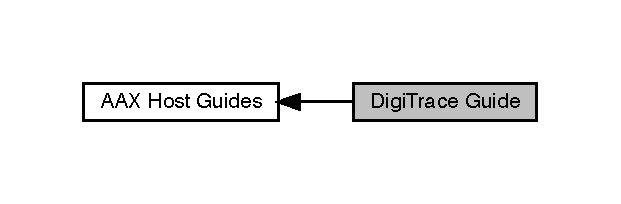
\includegraphics[width=298pt]{a00834}
\end{center}
\end{figure}
